\section{Gerador}

O \texttt{Generator} tem, como função, recebendo parâmetros como comprimento,
largura, raio, etc., gerar ficheiros de texto com a extensão \verb|.3d|, cujo conteúdo
é a informação sobre as figuras a criar. 

Nesta secção ir-se-á descrever o processo de desenvolvimento das figuras
necessárias do sistema solar. As figuras pertinentes a desenhar são a esfera
(para os planetas e sol) e um disco (para alguns planetas que os tenham, como
por exemplo Saturno) e um bule que servirá de cometa. 



\subsection{Esfera}
%---------------------------------------------------------------------------------------------------------------%
\subsubsection{Vértices da geometria}
Para a construção da esfera teve-se que ter em conta coordenadas esféricas
modificadas para o referencial rodado com Y para cima, Z como eixo das abcissas
e X como eixo das ordenadas, como demonstra a Equação~\ref{eq:equ2}.


\begin{equation}
    \begin{cases}
    x = \cos(\phi) * \sin(\theta) * \rho \\
    y = \sin(\phi) * \rho \\
    z = \cos(\phi) * \cos(\theta) *\rho
    \end{cases}
\label{eq:equ2}
\end{equation}

Na Equação~\ref{eq:equ2}, $\rho$ representa o raio, $\phi$ o ângulo polar sendo
$\phi \in [-\dfrac{\pi}{2}, \dfrac{\pi}{2}]$, $\theta$ representa o ângulo
azimutal sendo $\theta \in [0, 2\pi]$. 

\subsubsection{Vetores normais à superfície da geometria}

Para a aplicação de luzes no \emph{Engine} é necessário efetuar o cálculo dos
vetores normais. O cálculo pode ser efetuado de diversas formas, tanto
computacionais, como o cálculo de derivadas com o cálculo do vetor normal dessas
derivadas (devidamente normalizado), podem ser obtidas por interpolação de
vértices, e se a geometria já for conhecida, analiticamente. A normalização
é necessária, uma vez que, a fórmula para o cálculo da intensidade da luz da lei
de \emph{Lambert}, que postula que a intensidade refletida por um material
puramente difuso é proporcional ao cosseno do ângulo entre a normal da
superfície e a direção da luz de entrada. Ora para computar o cosseno, pode-se
usa-se o produto externo, e tendo vetores unitários a computação é mais
eficiente. Outra questão é o facto de diferentes vetores em vértices de um mesmo
triângulo terem magnitudes diferentes, e o OpenGL computa as normais com
a interpolação, criando uma cópia dos vetores normais. Se os vetores estiverem
com a mesma magnitude, esse problema não se coloca, uma vez que estão
normalizados.

Assim, para o cálculo das normais de uma esfera sabemos as direções de cada
ponto, e para serem coordenadas de um vetor unitário basta o raio ser 1. Assim
a Equação~\ref{eq:norm1} representa o cálculo de uma normal de um vértice da
esfera.

\begin{equation}
    \begin{cases}
    N_x = \cos(\phi) * \sin(\theta) \\
    N_y = \sin(\phi) * \rho \\
    N_z = \cos(\phi) * \cos(\theta) 
    \end{cases}
\label{eq:norm1}
\end{equation}


\subsubsection{Coordenadas de texturas para a geometria}

Usando uma textura bidimensional, sabendo que as coordenadas da mesma do OpenGL
variam entre 0 e 1, pode-se cobrir um geometria descrevendo as coordenadas em
$x$ e $y$ desse referencial. Pretende-se construir a esfera de cima para baixo,
desde $\frac{\pi}{2}$ a $-\frac{\pi}{2}$ do ângulo $\phi$. Se considerarmos uma
textura orientada como um retrato, a primeira coordenada de $x$ será
0 e a primeira coordenada de $y$ será 1, e pretende-se que o valor de $x$
aumente da esquerda para direita, e diminua de cima para baixo, e o valor de $y$
diminua de cima para baixo.

\newpage
\subsubsection{Diagrama}


\begin{center}
 	
 	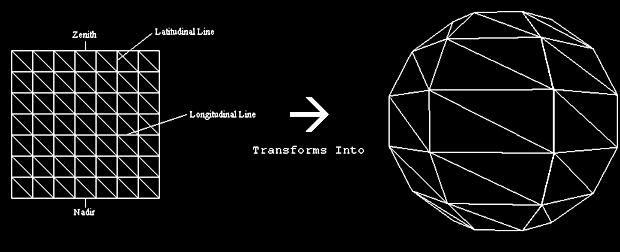
\includegraphics[width=\textwidth,height=\textheight,keepaspectratio]{resources/sphere05.jpg}
 	\captionsetup{type=figure, width=0.8\linewidth}
	\caption{Objetivo do algoritmo de construção de esfera}
\label{fig:ssec1:diagram:plane:to:sphere} 
\end{center}



\begin{center}
 	
 	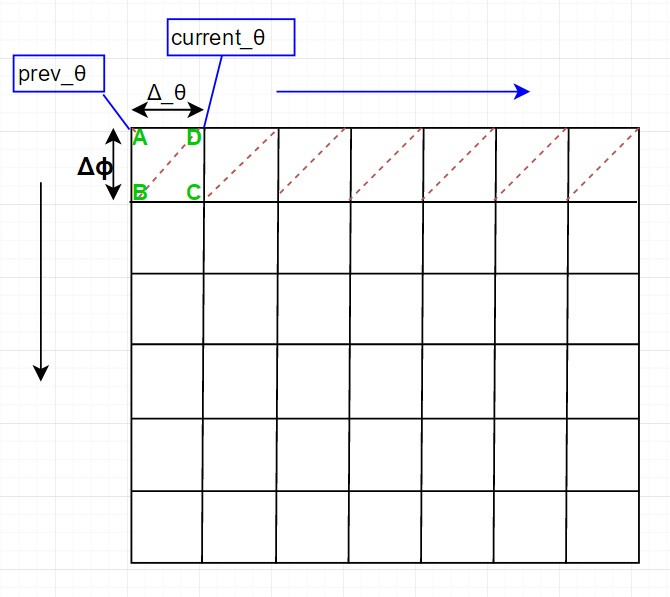
\includegraphics[keepaspectratio]{resources/esferaw.jpg}
 	\captionsetup{type=figure, width=0.8\linewidth}
	\caption{Diagrama de representativo de construção de esfera}
\label{fig:ssec1:diagram:sphere} 
\end{center}


No \emph{Figura~\ref{fig:ssec1:diagram:sphere}} pode-se ver uma matriz, que
representa a esfera nos graus de $\phi$ e $\theta$ para 6 \emph{stacks}
e 7 \emph{slices}. Assim como um mapa representativo da Terra, pretende-se
mostrar os pontos se a esfera fosse aplanada (ver
\emph{Figura~\ref{fig:ssec1:diagram:plane:to:sphere}}).

Em cada quadrícula são calculados 4 pontos iniciais, com base nos cálculos
apresentados pelo fórmula anterior. Note-se que, se usou duas variáveis para
guardar o $\phi$ anterior e o $\phi$ corrente, e $\theta$ anterior  e $\theta$
corrente. Adicionalmente é calculada a diferença de graus entre \emph{slices}
e \emph{stacks}, representados por $\Delta \phi$ e $\Delta \theta$,
respetivamente. Adicionalmente serão calculados os vetores normais, um por
vértice, como descrito na Equação~\ref{eq:norm1}.

A intenção é calcular cada quadricula para cada linha e coluna, com auxilio das
diferenças dos ângulos e à medida que se avança em cada quadricula, guardar
o último grau calculado ($\phi$ e $\theta$) e calcular nos pontos com
o incremento nestes ângulos. Assim desloca-se para a direita na matriz, conforme
$\theta$ avança de 0 para $2\pi$ e para baixo, conforme $\phi$ avança de
$\dfrac{\pi}{2}$ para $-\dfrac{\pi}{2}$ (sentido dos ponteiros do
relógio). Note-se que a Figura~\ref{fig:ssec1:diagram:sphere} pode representar
de igual modo, a elaboração das coordenadas das texturas, tendo em conta, que no
algoritmo, cada coluna tem que refletir o valor de $x$ e cada linha $y$ e, como
se pretende aplicar a textura de cima para baixo, terá que se subtrair cada
valor de linha ou coluna a 1, para as coordenadas decrescerem.




\newpage


\subsection{Disco}
Nesta secção descreve os procedimentos usados para desenvolver um disco.
A motivação para o desenvolvimento desta figura provém da necessidade de
representar os anéis que rodeiam os planetas Saturno e Úrano.


\subsubsection{Vértices da geometria}

Para criar um modelo do sistema solar é necessário criar discos para aplicar em
Saturno e, eventualmente, em Urano. Note-se que, todos os gigantes de gás
possuem anéis, no entanto, dado que os anéis de Júpiter e Neptuno são pequenos
não se considera a construção do mesmo.

Com efeito, requer-se para este projeto que se criem discos de vários tamanhos
para os anéis de Saturno e Urano. Note-se que cada anel tem que ter alguma
espessura, uma vez que, num plano, no \emph{OpenGL} não se consegue ver
o objeto. Assim cada disco terá duas circunferências, uma interior e outra
exterior, com raio interno e externo respetivamente. Assim, as duas
circunferências têm os mesmos pontos \emph{xx} e \emph{zz} mas com uma distancia
fixa no eixo \emph{yy}. 

A fórmula para desenhar uma circunferência está representada na
\emph{Equação~\ref{eq:equ3}}, podendo acrescentar a componente em $y$ para criar
um cilindro com uma altura pequena, mas suficiente para se poder distinguir.

\begin{equation}
\begin{cases}
			x =  \sin(\theta) * r \\
	    z =  \cos(\theta) * r
\end{cases}
\label{eq:equ3}
\end{equation}



Nesta secção apresentam-se diagramas que explicam o processo de criação de uma
disco.

A \emph{Figura~\ref{fig:ssec1:disc}} representa a forma como a iteração será
feita, bem como apresenta de lado a espessura do disco.


\begin{center}
 	
 	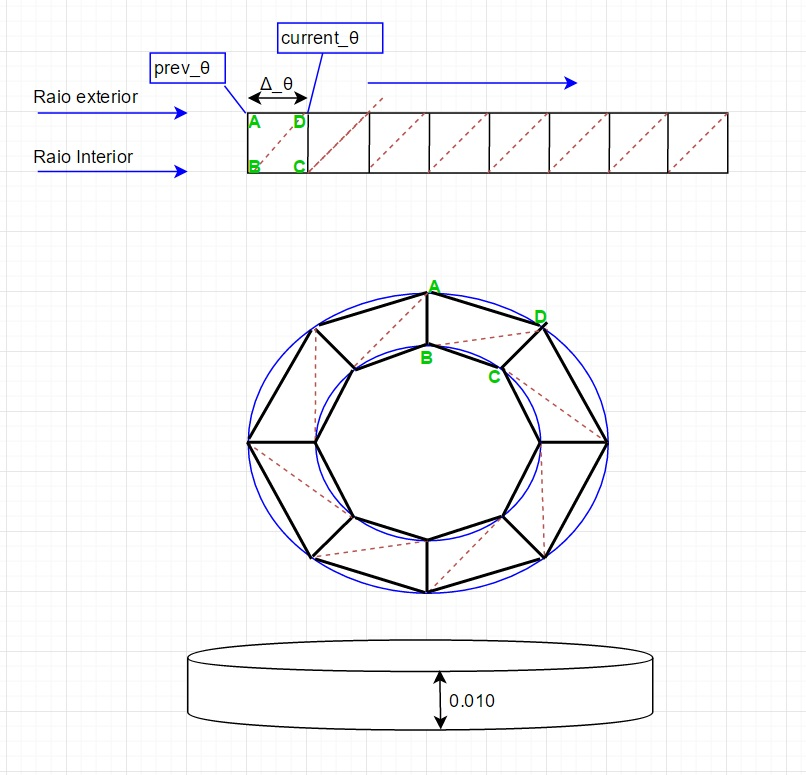
\includegraphics[width=\textwidth,height=\textheight,keepaspectratio]{resources/disco.jpg}
 	\captionsetup{type=figure, width=0.8\linewidth}
	\caption{Diagrama Disco}
\label{fig:ssec1:disc} 
\end{center}

Como se pode verificar o diagrama é relativamente semelhante ao da esfera.
A matriz aqui observada apenas tem uma linha porque não se consideram
\textit{stacks} na representação do disco. As 8 colunas que representam as
8 \textit{slices} (estas 8 slides servem meramente para propósitos
exemplificativos). 


\begin{center}
 	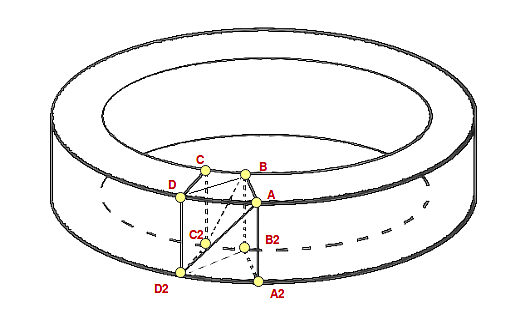
\includegraphics[width=\textwidth,height=0.5\textheight,keepaspectratio]{resources/discodiagram.png}
 	\captionsetup{type=figure, width=0.8\linewidth}
	\caption{Pormenor dos vértices para desenho de um disco}
\label{fig:sec1:disc:vertex} 
\end{center}

Tal como na esfera, pretende-se criar quadricula a quadricula, criando os
triângulos na orientação necessário, para a parte interior, exterior e os topos.


\subsubsection{Vetores normais à superfície da geometria}

À semelhança da esfera, podem-se obter os vetores normais do disco de forma
analítica, sendo que no topo superior o vetor normal terá as coordenadas (0,1,0)
e para o topo inferior terá as coordenadas (0,-1,0).

Para o cálculo dos vetores normais da circunferência exterior, pode-se aplicar
o mesmo principio da esfera, e usar as coordenadas da circunferência com raio 1. 
Para o lado interior, apenas é necessário mudar a direção dos vetores normais do
exterior. A Equação~\ref{eq:norm2} mostra a fórmula para as normais exteriores.


\begin{equation}
\begin{cases}
			N_x =  \sin(\theta) \\
	    N_z =  \cos(\theta) 
\end{cases}
\label{eq:norm2}
\end{equation}


\subsubsection{Coordenadas de texturas para a geometria}

A textura que se pretende aplicar é uma faixa horizontal, sendo que o lado de
fora do disco é o lado direito, e lado interior é o lado esquerdo, e que se
pretende repetir. Assim para as coordenadas de textura apenas é necessário
definir as coordenadas entre 0 e 1 para os topos, podendo aplicar-se uma pequena
porção de cada lado, para tapar a espessura do disco.

Assim, as coordenadas para os pontos definidos na
Figura~\ref{fig:sec1:disc:vertex} são:

\begin{itemize}

\item $A(1, 0)$
\item $B(0, 0)$
\item $C(0, 1)$
\item $D(1, 1)$
\item $A2(1, 0)$
\item $B2(0, 0)$
\item $C2(0, 1)$
\item $D2(1, 1)$

\end{itemize}


\subsection{\emph{Patch} de Bézier baseado em ficheiro de pontos de controlo}

\subsubsection{Vértices da geometria}

Para este projeto, requere-se que se obtenha pontos de controlo de uma
superfície de Bézier, através de uma ficheiro \emph{teapot.patch}, para
a construção de um bule de chá, para a representação de um cometa. O formato de
ficheiro é o que se segue:
\begin{enumerate}
	\item Número de \emph{patches};
	\item Índices para \emph{patches} (16 por linha, tantas linhas como nº de
		\emph{patches});
	\item Número de pontos de controlo;
	\item Ponto de controlo (coord.\ x, y, z) por linha, tantas linhas como nº de
		pontos de controlo;
\end{enumerate}



A função \texttt{drawPatch}, trata do processamento de leitura de transformação
dos valores lidos em ficheiro num vetor de \texttt{MatrixP}, onde por último,
para cada matriz armazenada no vetor anterior, para um valor de $i$ e um valor
de $j$ dividido pela tecelagem, iterando cada um desses valor entre 0 e o valor
da tecelagem, cria-se 4 pontos da superfície de Bézier, para cada iteração, onde
são retirados os triângulos e armazenados num ficheiro \.3d, todos os vértices
calculados.  Para calcular cada ponto da superfície de Bézier, é utilizada
a função \texttt{getBezierPatchPoint}, que recebe um valor de $u$, $v$ e uma
matriz de pontos de controlo. 

\newpage

Se se tiver um \emph{array} bi-dimensional de pontos
$P_{i,j}$, com $i\in[0, m]$, e $j\in[0,n]$, então pode-se
construir uma superfície Bézier da mesma forma usando um método similar a uma
curva cúbica de Bézier. Neste caso, ao invés de um parâmetro, existem dois
($u$ e $v$), onde $u\in[0,1]$ e $v\in[0,1]$.
Uma superfície de Bézier bi-cúbica (m=n=3), dado que tem por base curvas cúbicas
de Bézier definidas por 4 pontos de controlo, uma vez que é bi-dimensional, é definida por 16 pontos de
controlo $P_{i,j}$, e  representa-se pela \emph{Equação~\ref{eq:bezierpatch}}. Um
exemplo de uma superfície de Bézier está na \emph{Figura~\ref{fig:patchexample}} 

\begin{equation}
B(u,v)=\sum_{j=0}^{3}\sum_{i=0}^{3}B_{i}(u)P_{i,j}B{j}(v)
\label{eq:bezierpatch}
\end{equation}



\begin{center}
 	
 	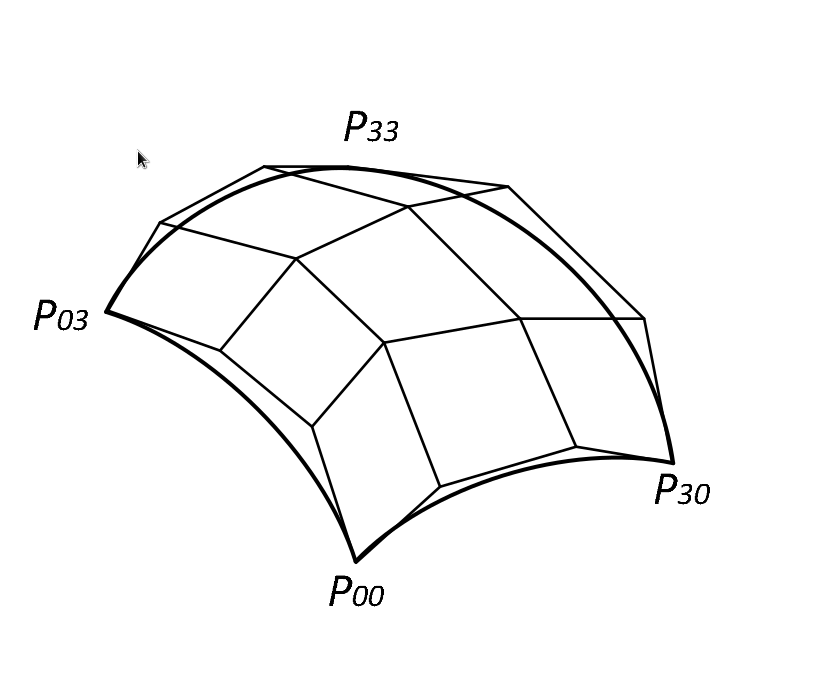
\includegraphics[width=0.5\textwidth,height=0.5\textheight,keepaspectratio]{resources/beziersupf.png}
 	\captionsetup{type=figure, width=0.8\linewidth}
	\caption{Superfície de Bézier bi-cúbica}
\label{fig:patchexample} 
\end{center}
Temos que:
\begin{gather*}
M = \begin{bmatrix}
-1 &  3 & -3 & 1  \\
 3 & -6 & 3  & 0  \\
-3 &  3 & 0  & 0  \\
1  &  0 & 0  & 0  \\
\end{bmatrix}
\end{gather*}

O parâmetros $u$ e $v$ estão entre 0 e 1, à semelhança do parâmetro $t$ da
função para uma curva de Bézier, onde $M$ é a matriz dos coeficientes obtida da
\emph{Equação~\ref{eq:beziercurve}}. A explicação para a obtenção de um ponto
numa superfície de Bézier, e, grosso modo, análoga à obtenção de um ponto numa
curva de Bézier, sendo que neste caso, estão dois parâmetros a variar entre
0 e 1, criando uma malha de com curvas de Bézier, conforme está na
\emph{Figura~\ref{fig:patchexample}}. Derivando
a \emph{Equação~\ref{eq:bezierpatch}} obtém-se
a representação matricial na \emph{Equação~\ref{eq:bezierpatchmatrix}}.

\begin{equation}
B(u,v) = \begin{bmatrix}
       u^{3} & u^{2} & u & 1          \\
		\end{bmatrix}
		M\begin{bmatrix}
		       P_{00} & P_{01} & P_{02} & P_{03}   \\
		       P_{10} & P_{11} & P_{12} & P_{13}   \\
		       P_{20} & P_{21} & P_{22} & P_{23}   \\
		       P_{30} & P_{31} & P_{32} & P_{33}
		     \end{bmatrix}
		M^{T} \begin{bmatrix}
		       v^{3} \\
		       v^{2} \\
		       v \\
		       1
		     \end{bmatrix}
\label{eq:bezierpatchmatrix}				 
\end{equation}

\paragraph{Função \texttt{getBezierPatchPoint}}

Antes de descrever a função \texttt{getBezierPatchPoint} é necessário descrever
algumas funções cridas par utilizar nessa função. 

Para cálculos com valores escalares de vírgula flutuante, nomeadamente
multiplicação de matrizes, criou-se a função \texttt{multMatrix} que multiplica
duas matrizes. Para obter um cálculo correto, são obtidas as dimensões das
matrizes (nº de linhas e nº de colunas), tal que, as dimensões para uma dada
matriz M1 são m $\times$ n, e as dimensões para uma dada 
matriz M2 são p $\times$ q. Para obtenção da matriz resultado, tem-se em conta
o nº de linhas da matriz M1 (m) e o nº de colunas da matriz M2 (q), onde
a matriz resultante terá um dimensão m $\times$ q. Note-se que os valores n ---
nº de colunas da matriz M1 --- e p --- nº de linhas da matriz M2 têm que ser
iguais. No entanto, essa verificação não é feita no código, no entanto,
assume-se que o programador sabe da especificação desta função. Para guardar
o valor da multiplicação de matrizes (somatório da multiplicação das linhas com
as colunas), usa-se um acumulador de resultado, fazendo variar um índice k,
entre 0 e p (que poderia ser n).

A função \texttt{matrixPointToScalar} obtém as coordenadas de x, ou de y, ou de
z, da matriz de pontos de controlo e armazena esses valores numa matriz de
escalares.


A função \texttt{getBezierPatchPoint} utiliza
a \emph{Equação~\ref{eq:bezierpatchmatrix}}, sendo o código amigável na sua
leitura e interpretação, uma vez que abstrai detalhes de implementação através
dos tipos de matrizes já mencionados. Em primeiro lugar,  a função calcula
a matriz U e a matriz V, com os parâmetros $u$ e $v$ respetivos, conforme
a equação. A segunda parte do algoritmo é multiplicar a matriz U por M, e matriz
$M^T$ por V e guarda cada resultado numa matriz. Note-se que, $M = M^T$, então
a matriz M é reutilizada.

Para calcular o ponto da superfície de Bézier, é necessário obter cada
coordenada dos pontos de controlo, sendo que a matriz de escalares da coordenada
x será para calcular a coordenada x do ponto da superfície, a matriz de
escalares da coordenada y será para calcular a coordenada y do ponto da
superfície e  a matriz de escalares da coordenada z será para calcular
a coordenada z do ponto da superfície. Cada matriz de escalares é multiplicada
pelo resultado de $UM$, e o resultado desta, com o resultado de $M^{T}V$ ou $MV$.
As matrizes resultantes destas operações são matrizes com dimensão $1\times1$,
com cada valor da coordenada x, y e z do ponto da superfície. Essas coordenadas
são guardadas num \texttt{Point3d} que é retornado pela função. 

Os resultados da aplicação do algoritmo para uma tecelagem de 50 podem ser
vistos nas figuras abaixo.

\begin{center}	
 	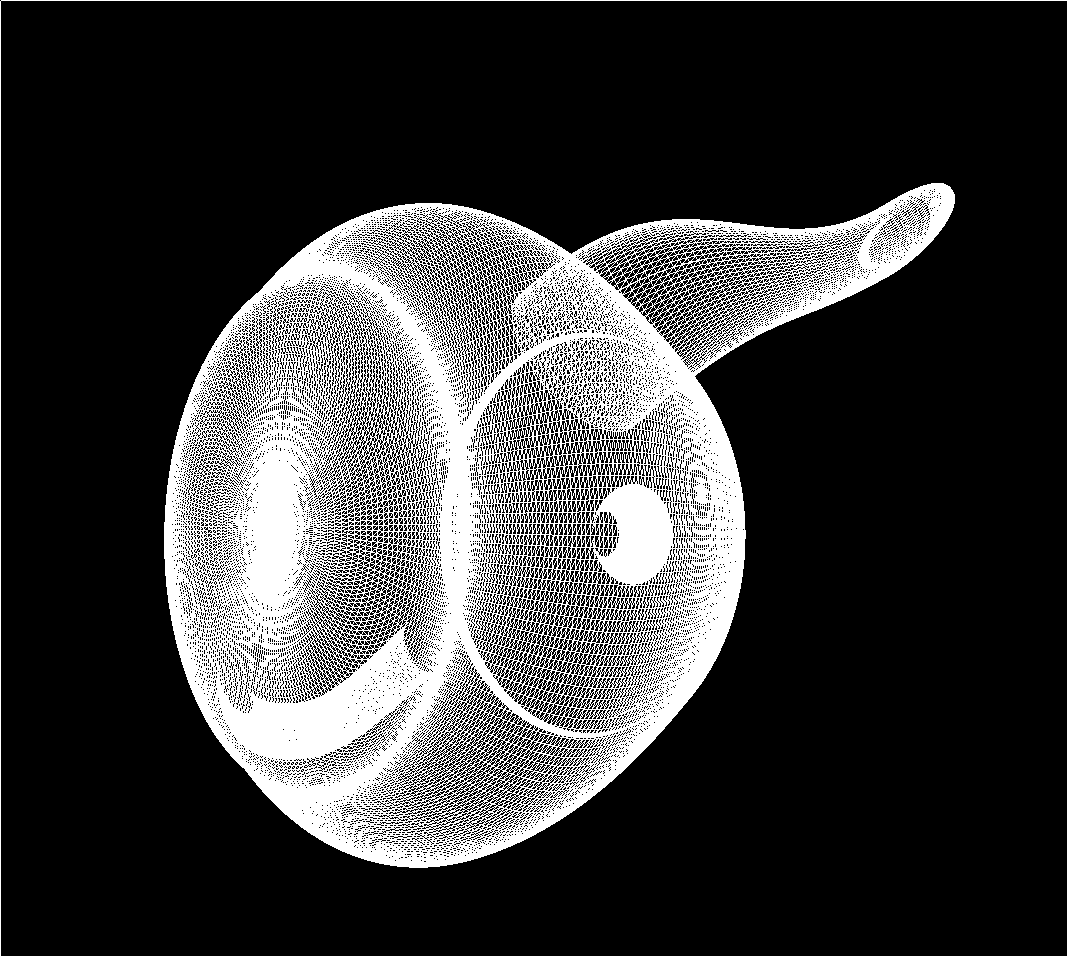
\includegraphics[width=\textwidth,height=\textheight,keepaspectratio]{resources/teapotBaixo.png}
 	\captionsetup{type=figure, width=0.8\linewidth}
	\caption{Bule visto de baixo}
\label{fig:teapotbottom} 
\end{center}

\begin{center}	
 	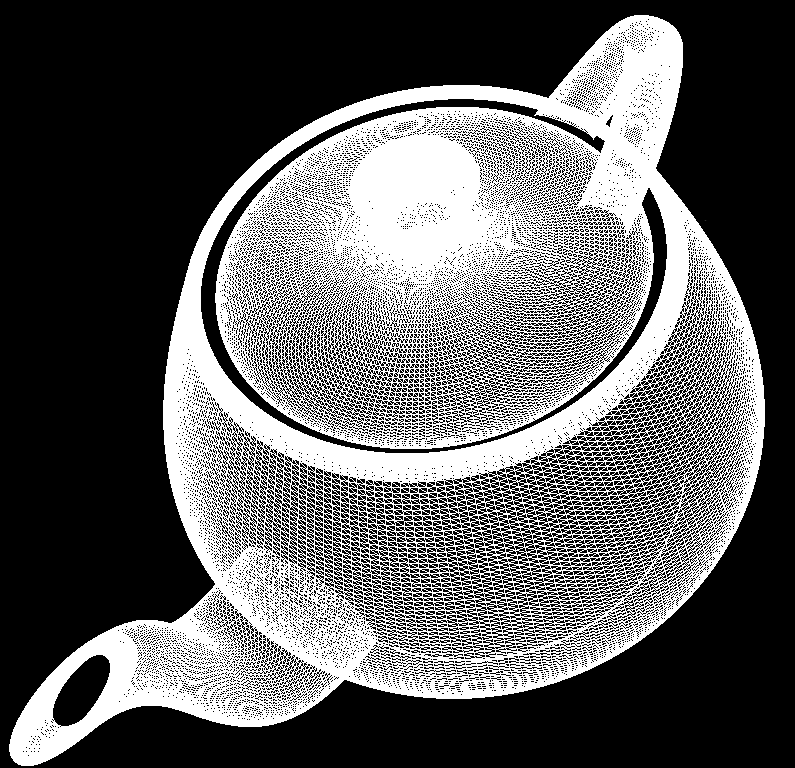
\includegraphics[width=\textwidth,height=\textheight,keepaspectratio]{resources/teapotCima.png}
 	\captionsetup{type=figure, width=0.8\linewidth}
	\caption{Bule visto de cima}
\label{fig:teapotabove} 
\end{center}


\begin{center}	
 	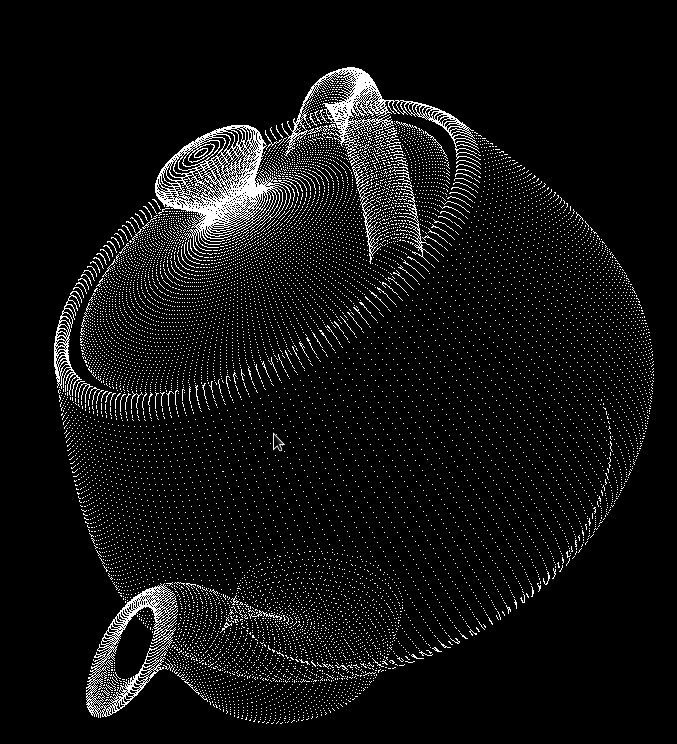
\includegraphics[width=\textwidth,height=\textheight,keepaspectratio]{resources/teapotPontos}
 	\captionsetup{type=figure, width=0.8\linewidth}
	\caption{Pontos da superfície do bule}
\label{fig:teapotpoints} 
\end{center}

\subsubsection{Vetores normais à superfície da geometria}


Para obter os vetores normais à superfície é preciso obter primeiro as tangentes
da superfície relativamente ao parâmetro $u$ e ao parâmetro $v$, ou seja
é preciso obter as derivadas parciais da superfície. Cada derivada representa
uma direção, ou um vetor, e representa a taxa de crescimento da função em
relação àquele parâmetro. As derivadas são tangentes à superfície. Para obter
cada derivada utiliza-se a Equação~\ref{eq:bezierdevu}
e a Equação~\ref{eq:bezierdevv}. 

Em seguida é necessário calcular o produto externo para obter o vetor diretor da
superfície no ponto da superfície, que se obtém a partir de $u$ e $v$ com as
funções anteriormente descritas. Este vetor não se encontra normalizado, pelo
é necessário dividir o vetor pela norma para obter um vetor unitário.

\begin{equation}
	\frac{\partial B(u,v)}{\partial u} = \begin{bmatrix}
       3u^{2} & 2u & 1 & 0          \\
		\end{bmatrix}
		M\begin{bmatrix}
		       P_{00} & P_{01} & P_{02} & P_{03}   \\
		       P_{10} & P_{11} & P_{12} & P_{13}   \\
		       P_{20} & P_{21} & P_{22} & P_{23}   \\
		       P_{30} & P_{31} & P_{32} & P_{33}
		     \end{bmatrix}
		M^{T} \begin{bmatrix}
		       v^{3} \\
		       v^{2} \\
		       v \\
		       1
		     \end{bmatrix}
\label{eq:bezierdevu}				 
\end{equation}

\begin{equation}
	\frac{\partial B(u,v)}{\partial v} = \begin{bmatrix}
       u^{3} & u^{2} & u & 1          \\
		\end{bmatrix}
		M\begin{bmatrix}
		       P_{00} & P_{01} & P_{02} & P_{03}   \\
		       P_{10} & P_{11} & P_{12} & P_{13}   \\
		       P_{20} & P_{21} & P_{22} & P_{23}   \\
		       P_{30} & P_{31} & P_{32} & P_{33}
		     \end{bmatrix}
		M^{T} \begin{bmatrix}
		       3v^{2} \\
		       2v \\
		       1 \\
		       0
		     \end{bmatrix}
\label{eq:bezierdevv}				 
\end{equation}

A função \texttt{getPartialDerivativeBezierPatchPointParamU} aplica
a Equação~\ref{eq:bezierdevu} e a função
\texttt{getPartialDerivativeBezierPatchPointParamV} aplica
a Equação~\ref{eq:bezierdevv} e o algoritmo destas duas funções é similar
à função \texttt{getBezierPatchPoint}, exceto nos valores dos vetores da
derivada $U$ e $V$, e no tipo de dados que devolve. A função
\texttt{getNormalBezierPatchPoint} aplica as duas funções mencionadas, calcula
o o produto externo, normalizando depois o vetor. Note-se que, pode ocorrer que
o vetor seja nulo, devido a descontinuidades, ou onde a derivada é 0, ou as
derivas têm o mesmo valor.
Daí que não se normalize esses vetores, pelo que é devolvido o vetor nulo.

\subsubsection{Coordenadas de texturas para a geometria}

Para as coordenadas de textura usou-se os valores de $u$ e $v$ para definir as
mesmas.
